\section{Ejercicio 3}

\subsection{Descripción del problema}

\subsubsection{Enunciado Informal}

En este problema se nos presenta un conjunto de ciudades con rutas entre las mismas que pueden o no estar ya construidas y tienen un costo de construccion/destrucción dependiendo de si ya existen. Se debe destruir y construir rutas tal que haya una sola forma de llegar de una ciudad a cualquier otra (se puede pasar por ciudades intermedias).Se debe tratar de minimzar el costo de conseguir este objetivo.

\subsubsection{Enunciado Formal}

Se tiene un conjunto de vertices y aristas que conectan a algunos de estos vertices entre si. Para cada par de vertices existen un número asignado el cual es el costo de agregar/eliminar la arista que conecta estos 2 vecrtices. El objetivo es encontrar el minimo coste necesario para lograr que el grafo resultante sea un arbol de expansión.\\
Esto es equivalente al enunciado orginal porque los vertices son las ciudades, los caminos son las aristas y la definición de arbol de expansión es un árbol que incluya todos los vertices del grafo (y la definición de árbol es que haya exctamente una única manera de llegar de un vertice a cualquier otro del mismo).

\subsubsection{Formato de entrada y salida}
La entrada esta conformada por:\\
una línea con un entero N con la cantidad de ciudades;\\
N*(N-1)/2 lineas describiendo como estan comunicados 2 ciudades.
Estas lineas estan formados por 2 enteros C1 y C2 indicando la conexión entre que par de vertices se está describiendo, seguido de un entero E indicando si la ruta existe y un entero P indicando el costo de construcción/destrucción de la ruta.\\
La salida es una unica linea con un entero indicando el minimo costo requerido para lograr el objetivo, seguido de un entero con la cantidad de rutas que forman parte de la solución y la lista de rutas que forman parte de la solución descriptas como un par de enteros que indican el par de ciudades que esa ruta conecta

\subsubsection{Ejemplo con Solucion}
Ejemplo:un ejemplo en que no queda ningun elemento sin pintar\\
Entrada:\\
4\\
0 1 0 3\\
0 2 0 1\\
1 2 1 2\\
0 3 0 6\\
1 3 1 4\\
2 3 1 1\\
Salida:\\
2 3 0 3 1 3 0 2\\
Explicacion:\\
Como 1 2 y 3 forman un triangulo con todo conectado necesariamente se debe eliminar una arista. Se elimará la mas barata ya que el objetivo es simplemente incluir todos los elementos con el menor costo posible. Asi que no conviene gastar en eliminar demás ni en agregar en exceso. Si que es necesario elminar exactamente 1 y esa sería la arista mas barata (es decir la de costo 1. De manera similar el vertice 0 quedo aislado del grafo y debe comunicarse usando el camino mas corto posible el cual tiene costo 1.




\subsection{Explicación de la solución}

Para resolver este problema es importante notar que si divido el grafo original en sus componentes conexas, se puede notar que las únicas operaciones permitidas serían eliminar aristas dentro de cada componente o agregar para conectar las componentes. Es obvio que las compnentes al ser conexas no tienen caminos conectandolas por lo cual es obvio que solo se puede agregar aristas por lo tanto lo único que sería demostrar es la otra afimación\\
 Esto es así ya que agregar aristas dentro de un mismo componente lo único que hace es agregar mas aristas a las posibles para eliminar, ya que se crean caminos alternativos y agrega aristas al total. Esto en principio podría ser positivo ya que podría haber una combinación de agregar una arista y eliminar 2 que sea más óptima que eliminar una sola. Sin embargo, esto no es asi ya que al agregar aristas únicamente se permite eliminar aristas que comunican 2 vertices que previamente estaban comunicados con un conjunto de caminos que tienen exactamente una arista que se encuentra en todos los caminos (pero con la arista extra tienen caminos alternativos que no usan dicha arista), ya que caulquier otra arista ya anteriormente podía ser eliminada. Es decir 2 conjuntos de vertices cada uno de los cuales tienen al menos 2 caminos entre cada par de vértices del mismo pero solo uno a los del otro conjunto. Si se agrega una arista dentro de un conjunto este no se ve afectado (de la misma manera si agrega una con alguno fuera de estos conjuntos no se crea ningún camino alternativo), pero si se agreaga una arista comunicando los 2 conjuntos distintos se crea la posibilidad de elegir alguno de los 2 caminos comunicando los conjuntos. Como cada arista agregada solo puedo afectar a un par de estos conjuntos (ya que ninguna pueda estar afuera) a lo sumo es posible crear un camino nuevo. En caso de que el camino orignal este formado por varios elementos se sabe que debe esta formado por todas aristas que no tienen otra forma de comunicarse a la totalidad de los vertices sin usar dicho camino ya que si lo hubiera existiría otro camino alternativo entre los 2 conjuntos originales. Por lo tanto solo es posible eminar una arista de dicho camino. Por lo tanto al agregar una arista se debe eliminar una arista extra para mantener el total pero se permite eliminar a lo sumo 1 arista que previamente no podía serlo. En conclusión se debe seguir elimando la misma cantidad de aristas de las originales y solo se aumenta el costo total agregando y elminando una demás \\
Entonces ya sabiendo que solo se puede realizar esas operaciones el problema se redujo en varios subproblemas en lo que se debe formar su arbol de máxima expansión ya que de esa manera se minimiza el costo de las aristas no usadas. Esto se puede hacer en pasos consistenes en agreagar a dicho arbol la arista de maximo tamaño posible en cada paso que no conecte vertices previamente conectados. Esto es exactamente lo que hace el algoritmo de kruskal \url{https://es.wikipedia.org/wiki/Algoritmo_de_Kruskal} el cuál será implementado teniendo un arreglo ordenado de forma decreciente con todas las aristas destruibles de la componente conexa con la que se esta trabajando. Al agregar una arista a dicho arbol es importante guardar cual fue la arista agregada para así poder reconstruir la solución para la salida. Cuando no se agrega una arista porque comunica 2 vertices ya previamente conectadas se le suma el valor correspondiente al costo total de las obras. Notese que se puede trabajar directamente con otdas las componentes fuertemente conexas a la vez en el mismo arreglo ya que simplemente haría que se vaya trabajando con cada subproblema por partes ya que no estan comunicados de ninguna manera\\
Ahora solo quedaría conectar todas dichas componentes. Para hacer eso se debe hacer un arbol que conecte la otdalidad de los nodos tratando de minimizar el costo. Para hacer esto también se podra usar kruskal pero suponiendo que cada una de las componentes conexas ya estan conectadas y cada una forman su propio conjunto en el algooritmo (sería parecido a empezar el algoritmo por la mitad del mismo). Para hacer esto se tomará las aristas construibles y se colocaran en un arreglo ordenado de forma creciente de tal manera que en cada paso se tome la de menor costo y se agregará al arbol generador final en caso que conecte 2 verticces que previamente no estaban comunicados entre si. De la misma forma que en el caso anterior cada vez que se agrega una arista se aumentariá el costo total y guardará la arista agregada para reconstruir la solución\\


Para el psudocodigo se utilizará la función sort que ordena el vector dado de menor a mayor o mayor a menor. La misma tiene complejidad en el peor caso de N*log(N) ya que la misma en las biblotecas standard por mas que varíen implementación deben garantizar un peor caso de N*log(N). Luego de leer la entrada lo cual se hace en tiempo O(1) para cada una de las n*(n-1)/2 lineas (ya que solo se debe colocar la información en el vector conrrespondiente), se procederá a resolver el problema con la información correspondiente ya colocada en los vectores destruction y construction (de acuerdo si el camino ya existe o no) guardando en cada una la tupla formada por c1, c2 y costo P. Por lo tanto construction como destruction pueden tener a lo sumo un elemento por linea de codigo por lo cual pueden tener a lo sumo O(N*N) elementos. Además es importante mencionar que de utilizará una clase llamada disjoint set que es un conjunto de elementos divido en varios subconjuntos implementada utilizando union find \url{https://en.wikipedia.org/wiki/Disjoint-set_data_structure} la implentación usada tiene complejidad de O(N) tanto para construirse, destruirse, hacer el find y el union.Por lo tanto el pseudocodigo quedaría:



	\algoritmo{MenorCosto}{entero n, $vector<tupla<entero, entero, entero>> construction$, $vector<tupla<entero, entero, entero>> destruction$}{}{\bigo($N*N*log(N)$)}{
	
\State sortcreciente(construction)\comment \bigo($N*N*log(N)$)
	\State sortdecreciente(destruction)\comment \bigo($N*N*log(N)$)
	\State Crear DisjointSet UDS de tamaño N \comment \bigo($N$)
	
\State Minimo $\gets$ 0 \comment \bigo($1$)
\State $vector<tupla<entero, entero>> solucion$
\For {i $\gets destruction[0],destruction[1],...,destruction[tamano(destruccion)-1]$} \comment se repite a lo sumo N*N veces
\State v1 $\gets$ i[0] \comment \bigo($1$)
\State v2 $\gets$ i[1] \comment \bigo($1$)

\If {$UDS.find(v1)\neq UDS.find(v2)$} \comment \bigo($N$)
	\State $UDS.setUnion(v1, v2)$; \comment \bigo($N$)
	\State Agregar $(v1,v2)$ al vector solucion  \comment \bigo($1$)
\EndIf
\If {$UDS.find(v1) = UDS.find(v2)$} \comment \bigo($N$)
	\State Minimo $\gets$ $Minimo-i[3]$; \comment \bigo($1$)
\EndIf

\EndFor

\For {i $\gets construction[0],construction[1],...,construction[tamano(construccion)-1]$} \comment se repite a lo sumo N*N veces
\State v1 $\gets$ i[0] \comment \bigo($1$)
\State v2 $\gets$ i[1] \comment \bigo($1$)

\If {$UDS.find(v1)\neq UDS.find(v2)$} \comment \bigo($N$)
	\State $UDS.setUnion(v1, v2)$; \comment \bigo($N$)
	\State Agregar $(v1,v2)$ al vector solución \comment \bigo($1$)
	\State Minimo $\gets$ $Minimo-i[3]$;\comment \bigo($1$)
\EndIf
\EndFor
	
\State la solución es Minimo seguido de n-1 y por ultima el contenido del vector solución escribiendo los elementos de cada par uno despues del otro.   
   
 
}{\bigo(N*N*log(N)) + \bigo(N*N)+\bigo(N*N)$=$\bigo(N*N*log(N))}


\subsection{Experimentación}
La experimentación del ejercicio 3 se llevó a cabo armando un grafo completo completo de n nodos. Las aristas se generaron desde (v1, v2), (v2, v3), ..., (v2, v3), (v3, v4), ..., (v(n-1), v(n-2)). Los costos son completamente aleatorios en cada instancia generada, para demostrar que no afectan los tiempos de ejecución, y para asignarle una densidad al grafo, se ordenó la lista de incidencia de manera aleatoria y se tomaron los max m * densidad primeros elementos de la mismas.\\
 
La principal observación que se puede realizar para este algoritmo es que los tiempos de ejecución dependen enteramente de la cantidad de vértices. La dependencia en N es visible en el cálculo de complejidad, pero se puede corroborar que cualquier variación de instancias no modifica los tiempos de ejecución. Para esto variamos la densidad del grafo, tomando aristas y costos de construcción completamente aleatorios para cada una, pero con N fijo. Esto nos da una distribución normal lo que nos permite corroborar que ninguna otra característica del grafo afecta los tiempos de ejecución:\\


\begin{figure}[!htb!]
	\begin{center}
		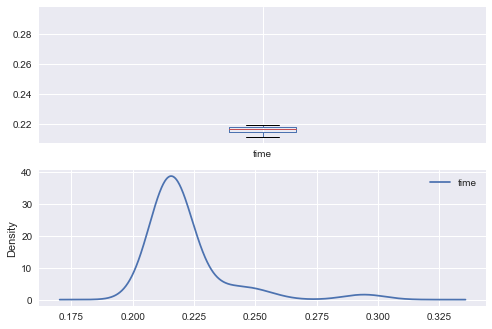
\includegraphics[width=300pt]{Imagenes/density.png}
		\caption{{\small \textit{densidad}}}
	\end{center}
\end{figure}


